% Provenance (never printed): cycle 4 (geographie and SVT, "La planete Terre"):
% why a flat map distorts, projections, scale, topographic maps and
% profiles, satellite images and satellite positioning; see
% sources/book1/PROVENANCE.md. Book 1, grade 9, chapter 5.
% Vocabulary guard: owns map projection (Mercator, equal-area), numerical
% scale and scale bar, topographic map, contour line and contour interval,
% remote sensing and satellite image, satellite positioning. "Scale" itself
% is g2's (drawing-to-map, Sync 1 ruling); globe and world map are g3's;
% parallels, meridians, latitude and longitude are g6's; altitude, relief
% and physical map are g4's; slope as a percentage was used in g9.2. The
% speed of light is the physics books' (recalled in prose). The V-rule of
% geological maps belongs to Book 3.
\chapter{Maps of the Whole Earth}\label{ch:g9:maps-of-the-earth}

On many classroom wall \omterm{def:g2:drawing-to-map:map}{maps}, Greenland looks about as big as Africa. On a
\omterm{def:g3:continents-and-oceans:globe}{globe}, Africa is about fourteen times larger: about 29~million square
kilometres for the African mainland, against about 2.1~million for
Greenland. Both are true pictures of the Earth, made with care. So which
one is lying, and why?
% ledger: data:ne-land (areas computed in figdata/grade-9/projections.py)

\begin{recall}
A \omterm{def:g2:drawing-to-map:map}{map} is a drawing of a place seen from above, smaller than the place, with
a \omterm{def:g2:drawing-to-map:legend}{legend} and a \omterm{def:g2:drawing-to-map:scale}{scale} (\cref{ch:g2:drawing-to-map}). A \omterm{def:g3:continents-and-oceans:globe}{globe} is a small
model of the round Earth; a \omterm{def:g3:continents-and-oceans:world-map}{world map} shows the whole Earth flat, in one
picture (\cref{ch:g3:continents-and-oceans}). \omterm{def:g6:latitude-longitude:latitude}{Parallels} and \omterm{def:g6:latitude-longitude:longitude}{meridians} give
every place its \omterm{def:g6:latitude-longitude:latitude}{latitude} and \omterm{def:g6:latitude-longitude:longitude}{longitude} (\cref{ch:g6:latitude-longitude}).
\omterm{def:g4:world-physical-map:altitude}{Altitude} is the height above \omterm{def:g4:world-physical-map:altitude}{sea level}, and a \omterm{def:g4:world-physical-map:physical-map}{physical map} shows the
\omterm{def:g4:world-physical-map:relief}{relief} in colours (\cref{ch:g4:world-physical-map}). In physics, you learn
that light travels at about \qty{300000}{km} per second.
\end{recall}
% ledger: const:c

\section{Why a flat map has to distort}

Try to flatten the peel of an orange on a table: it tears or it stretches.
The surface of a sphere cannot be laid flat without changing some lengths.
To draw the whole Earth on a sheet, a mapmaker chooses a rule that sends
every point of the \omterm{def:g3:continents-and-oceans:globe}{globe} to a point of the sheet, and chooses what the \omterm{def:g2:drawing-to-map:map}{map}
will keep true, and what it will give up.

\begin{definition}[Map projection]\label{def:g9:maps-of-the-earth:projection}
A \emph{map projection}\index{map projection} is a rule that sends every
point of the \omterm{def:g3:continents-and-oceans:globe}{globe}, given by its \omterm{def:g6:latitude-longitude:latitude}{latitude} and \omterm{def:g6:latitude-longitude:longitude}{longitude}, to a point of a
flat \omterm{def:g2:drawing-to-map:map}{map}. On a \emph{Mercator projection}\index{Mercator projection}, the
\omterm{def:g6:latitude-longitude:latitude}{parallels} and the \omterm{def:g6:latitude-longitude:longitude}{meridians} are straight lines crossing at right angles,
and the shape of every small region is kept, but areas are enlarged more
and more towards the \omterm{def:g3:continents-and-oceans:poles}{poles}. On an \emph{equal-area
projection}\index{equal-area projection}, every region keeps its true
area compared with the others, but shapes are bent, more and more towards
the edges of the \omterm{def:g2:drawing-to-map:map}{map}.
\end{definition}

The figure below draws the same equal circles on the \omterm{def:g3:continents-and-oceans:globe}{globe}, all of the same
size, onto both \omterm{def:g2:drawing-to-map:map}{maps}. On the Mercator \omterm{def:g2:drawing-to-map:map}{map}, the circles stay round but grow
towards the \omterm{def:g3:continents-and-oceans:poles}{poles}: at \omterm{def:g6:latitude-longitude:latitude}{latitude} \ang{60}, their area is four times what it
is at the \omterm{def:g3:continents-and-oceans:equator}{equator}, and near Greenland's middle, at about \ang{72}, about
ten times. On the equal-area \omterm{def:g2:drawing-to-map:map}{map}, the circles all keep the same area, but
those far from the centre are squashed into ovals.
% ledger: data:ne-land (circles and factors computed in figdata/grade-9/projections.py, mercator_area_factor)

No projection is the best for everything. The \omterm{def:g9:maps-of-the-earth:projection}{Mercator projection} was made
for sailors: a course that keeps the same compass direction is a straight
line on it. To compare the sizes of countries, of forests or of \omterm{def:g5:weather-and-climate:desert}{deserts}, an
equal-area \omterm{def:g2:drawing-to-map:map}{map} tells the truth. Before trusting a \omterm{def:g3:continents-and-oceans:world-map}{world map}, it is worth
asking which projection it uses.

\begin{omfigure}
\begin{tikzpicture}
\begin{axis}[name=merc, x=0.0215cm, y=0.0215cm, xmin=-180, xmax=180,
  ymin=-140, ymax=169, axis line style={black!50}, ticks=none,
  title={\footnotesize Mercator projection}, title style={yshift=-1ex}]
  \addplot[black!15, line width=0.3pt] table {figdata/out/grade-9-projections-merc-grid.dat};
  \addplot[fill=black!25, draw=black!45, line width=0.15pt] table {figdata/out/grade-9-projections-merc-land.dat};
  \addplot[fill=orange!55, draw=orange!70!black, line width=0.3pt] table {figdata/out/grade-9-projections-merc-greenland.dat};
  \addplot[fill=blue!30, draw=blue!60!black, line width=0.3pt] table {figdata/out/grade-9-projections-merc-africa.dat};
  \addplot[red!80!black, line width=0.6pt] table {figdata/out/grade-9-projections-merc-circles.dat};
\end{axis}
\begin{axis}[at={(merc.east)}, anchor=west, xshift=0.3cm, x=0.025cm, y=0.025cm,
  xmin=-165, xmax=165, ymin=-83, ymax=83, hide axis,
  title={\footnotesize an equal-area projection}, title style={yshift=-1ex}]
  \addplot[black!15, line width=0.3pt] table {figdata/out/grade-9-projections-moll-grid.dat};
  \addplot[fill=black!25, draw=black!45, line width=0.15pt] table {figdata/out/grade-9-projections-moll-land.dat};
  \addplot[fill=orange!55, draw=orange!70!black, line width=0.3pt] table {figdata/out/grade-9-projections-moll-greenland.dat};
  \addplot[fill=blue!30, draw=blue!60!black, line width=0.3pt] table {figdata/out/grade-9-projections-moll-africa.dat};
  \addplot[red!80!black, line width=0.6pt] table {figdata/out/grade-9-projections-moll-circles.dat};
\end{axis}
\end{tikzpicture}

{\small The same world on two projections. Red: circles of the same size on
the \omterm{def:g3:continents-and-oceans:globe}{globe}, centred every \ang{30} of \omterm{def:g6:latitude-longitude:latitude}{latitude} and \ang{60} of \omterm{def:g6:latitude-longitude:longitude}{longitude}.
Orange: Greenland; blue: the African mainland. On the Mercator \omterm{def:g2:drawing-to-map:map}{map} (left,
cut at \ang{80}\,S and \ang{84}\,N, since the \omterm{def:g3:continents-and-oceans:poles}{poles} would be infinitely
far), the two look about the same size; on the equal-area \omterm{def:g2:drawing-to-map:map}{map} (right), Africa
is about 14 times larger, as on the \omterm{def:g3:continents-and-oceans:globe}{globe}. Coastlines from Natural Earth.}
% ledger: data:ne-land
\label{fig:g9:maps-of-the-earth:projections}
\end{omfigure}

\begin{example}[Greenland and Africa]
Africa's mainland covers about 29~million~\unit{km^2}, Greenland about
2.1~million~\unit{km^2}: $29 \div 2.1 \approx 14$. Africa straddles the
\omterm{def:g3:continents-and-oceans:equator}{equator}, where the \omterm{def:g9:maps-of-the-earth:projection}{Mercator projection} hardly enlarges anything, while
most of Greenland lies between about \ang{60} and \ang{84} north, where
areas are enlarged from 4 to more than 10 times. On the Mercator \omterm{def:g2:drawing-to-map:map}{map}, the
two come out about the same size.
\end{example}
% ledger: data:ne-land (areas and ratios computed in figdata/grade-9/projections.py, areas)

\section{Scale}

A \omterm{def:g2:drawing-to-map:map}{map} of a \omterm{def:g1:landscapes-around-us:landform}{valley} or a town is so small a piece of the Earth that the
projection hardly matters. What matters is how much smaller than the
ground the \omterm{def:g2:drawing-to-map:map}{map} is.

\begin{definition}[Numerical scale and scale bar]\label{def:g9:maps-of-the-earth:numerical-scale}
The \emph{numerical scale}\index{numerical scale} of a \omterm{def:g2:drawing-to-map:map}{map} is a ratio such
as $1 : 25\,000$: one centimetre on the \omterm{def:g2:drawing-to-map:map}{map} stands for \num{25000}
centimetres on the ground, and the same for any unit. A \emph{scale
bar}\index{scale bar} is a ruler drawn on the \omterm{def:g2:drawing-to-map:map}{map}, marked with the
distances on the ground.
\end{definition}

\begin{method}[Using a numerical scale]
\begin{enumerate}
  \item Measure the distance on the \omterm{def:g2:drawing-to-map:map}{map}, in centimetres.
  \item Multiply it by the number after the colon: the result is the
        distance on the ground, in centimetres.
  \item Convert: divide by 100 for metres, by \num{100000} for kilometres.
\end{enumerate}
\end{method}

\begin{example}[A walk on a $1 : 25\,000$ map]
On a \omterm{def:g2:drawing-to-map:map}{map} at $1 : 25\,000$, a footpath measures \qty{6}{cm}. On the ground,
it is $6 \times 25\,000 = \num{150000}$~cm, that is \qty{1500}{m} or
\qty{1.5}{km}. Each centimetre of the \omterm{def:g2:drawing-to-map:map}{map} stands for \qty{250}{m}.
\end{example}

The \omterm{def:g9:maps-of-the-earth:numerical-scale}{scale bar} has one advantage over the \omterm{def:g9:maps-of-the-earth:numerical-scale}{numerical scale}: when a \omterm{def:g2:drawing-to-map:map}{map} is
enlarged or shrunk on a screen or a copier, the bar is enlarged or shrunk
with it and stays right, while the ratio printed in the corner becomes
wrong.

\section{The topographic map}

A \omterm{def:g4:world-physical-map:physical-map}{physical map} shows the \omterm{def:g4:world-physical-map:relief}{relief} with colours. A \omterm{def:g2:drawing-to-map:map}{map} of a small area shows
it far more precisely, with lines.

\begin{definition}[Topographic map]\label{def:g9:maps-of-the-earth:topographic-map}
A \emph{topographic map}\index{topographic map} is a detailed \omterm{def:g2:drawing-to-map:map}{map} of a
small area, at a \omterm{def:g2:drawing-to-map:scale}{scale} such as $1 : 25\,000$ or $1 : 50\,000$, that shows
the shape and the height of the ground, with the \omterm{def:g1:landscapes-around-us:water}{rivers}, roads, paths,
buildings and woods.
\end{definition}

\begin{definition}[Contour line and contour interval]\label{def:g9:maps-of-the-earth:contour}
A \emph{contour line}\index{contour line} is a line on a \omterm{def:g2:drawing-to-map:map}{map} joining
points of the ground at the same \omterm{def:g4:world-physical-map:altitude}{altitude}. The \emph{contour
interval}\index{contour interval} is the difference in \omterm{def:g4:world-physical-map:altitude}{altitude} between
two neighbouring contour lines; it is the same all over the \omterm{def:g2:drawing-to-map:map}{map}.
\end{definition}

Imagine a \omterm{def:g1:landscapes-around-us:landform}{hill} sliced by horizontal planes, one every \qty{100}{m}. Each
slice cuts the \omterm{def:g1:landscapes-around-us:landform}{hill} along a closed line; seen from above, these lines are
the \omterm{def:g9:maps-of-the-earth:contour}{contour lines}.

\begin{omfigure}
\begin{tikzpicture}[font=\footnotesize]
  % side view
  \fill[black!13] (0,0) .. controls (1.2,0.3) and (2.0,1.3) .. (2.8,2.2)
     .. controls (3.2,2.6) and (3.5,2.6) .. (3.7,2.2) .. controls (3.9,1.6) and (4.1,0.4) .. (4.5,0) -- cycle;
  \draw[black!70] (0,0) .. controls (1.2,0.3) and (2.0,1.3) .. (2.8,2.2)
     .. controls (3.2,2.6) and (3.5,2.6) .. (3.7,2.2) .. controls (3.9,1.6) and (4.1,0.4) .. (4.5,0);
  \draw[black!70] (-0.3,0) -- (4.9,0);
  \foreach \y/\h in {0.6/100, 1.2/200, 1.8/300} {
    \draw[omContour, dashed] (-0.3,\y) -- (4.9,\y);
    \node[anchor=east, omContour] at (-0.3,\y) {\h~m};
  }
  \node[anchor=south] at (3.3,2.5) {seen from the side};
  \node[anchor=north] at (1.4,-0.05) {gentle west slope};
  \node[anchor=north] at (4.1,-0.05) {steep east slope};
  % map view
  \begin{scope}[xshift=8.4cm, yshift=1.3cm]
    \draw[omContour, line width=0.5pt] (0.25,0) ellipse (2.1 and 1.25);
    \draw[omContour, line width=0.5pt] (0.75,0.02) ellipse (1.3 and 0.9);
    \draw[omContour, line width=0.5pt] (1.05,0.04) ellipse (0.62 and 0.5);
    \fill (1.25,0.05) circle (0.04);
    \draw[black!60] (1.25,0.05) -- (2.9,-0.6) node[anchor=west, inner sep=1.5pt] {summit};
    \node[omContour, fill=white, inner sep=0.5pt] at (-1.85,0) {100};
    \node[omContour, fill=white, inner sep=0.5pt] at (-0.55,0) {200};
    \node[omContour, fill=white, inner sep=0.5pt] at (0.43,0) {300};
    \node[anchor=north] at (0.25,-1.35) {seen from above: the contour lines};
    \draw[->] (2.7,0.9) -- (2.7,1.4) node[above] {N};
  \end{scope}
\end{tikzpicture}

{\small A \omterm{def:g1:landscapes-around-us:landform}{hill} sliced every \qty{100}{m} (a sketch). Seen from above, each
slice gives a closed \omterm{def:g9:maps-of-the-earth:contour}{contour line} around the summit. Where the slope is
steep (east), the lines are close together; where it is gentle (west), they
are far apart.}
\label{fig:g9:maps-of-the-earth:slices}
\end{omfigure}

A \omterm{def:g9:maps-of-the-earth:topographic-map}{topographic map} is read with a few rules.
\begin{itemize}
  \item \omterm{def:g9:maps-of-the-earth:contour}{Contour lines} never cross: a point has only one \omterm{def:g4:world-physical-map:altitude}{altitude}.
  \item The closer the \omterm{def:g9:maps-of-the-earth:contour}{contour lines}, the steeper the slope; far apart, the
        ground is gentle; no line at all, it is nearly flat.
  \item Closed lines nested inside one another, rising inwards, mark a \omterm{def:g1:landscapes-around-us:landform}{hill};
        its top is often marked by a dot with its \omterm{def:g4:world-physical-map:altitude}{altitude}, a \emph{spot
        height}.
  \item Where a \omterm{def:g9:maps-of-the-earth:contour}{contour line} crosses a \omterm{def:g1:landscapes-around-us:landform}{valley}, it bends upstream, in a V
        that points towards the head of the \omterm{def:g1:landscapes-around-us:landform}{valley}.
  \item Every fifth line, the \emph{index contour}, is drawn thicker and
        labelled with its \omterm{def:g4:world-physical-map:altitude}{altitude}.
\end{itemize}

The slope of the ground between two points is the rise divided by the
horizontal distance, often written as a percentage. On the \omterm{def:g2:drawing-to-map:map}{map} below,
going north from the \omterm{def:g1:landscapes-around-us:water}{river}, the \qty{200}{m} and \qty{400}{m} contours on
line C--D are about \qty{0.75}{km} apart: the slope is about $200 \div 750
\approx 0.27$, or \qty{27}{\%}.
% ledger: (invented region: crossings 2.09 and 2.83 km from C, figdata/grade-9/varden_topo.py)

\begin{method}[Drawing a topographic profile]
\begin{enumerate}
  \item Draw the line of the profile on the \omterm{def:g2:drawing-to-map:map}{map}, from one end (C) to the
        other (D).
  \item Lay the straight edge of a strip of paper along the line; mark C,
        D, and every point where the line crosses a \omterm{def:g9:maps-of-the-earth:contour}{contour line}, with
        its \omterm{def:g4:world-physical-map:altitude}{altitude}.
  \item Draw a horizontal axis as long as C--D (the distances) and a
        vertical axis of \omterm{def:g4:world-physical-map:altitude}{altitudes}.
  \item Carry each mark to the graph, at its distance from C and at its
        \omterm{def:g4:world-physical-map:altitude}{altitude}, and join the points with a smooth curve: rounded on \omterm{def:g1:landscapes-around-us:landform}{hill}
        tops, flat along a \omterm{def:g1:landscapes-around-us:landform}{valley} floor.
\end{enumerate}
\end{method}

\begin{omfigure}
\begin{tikzpicture}
\begin{axis}[name=map, x=2cm, y=2cm, xmin=2, xmax=8, ymin=1.8, ymax=6.2, ticks=none,
  axis line style={black!60}, clip mode=individual]
  \addplot[contour] table {figdata/out/shared-region-contours.dat};
  \addplot[index contour] table {figdata/out/shared-region-index-contours.dat};
  \addplot[river] table {figdata/out/shared-region-river.dat};
  \addplot[only marks, mark=none, point meta=explicit symbolic, nodes near coords,
    nodes near coords align={center}, nodes near coords style={font=\tiny, fill=white, inner sep=0.6pt, text=omContour}]
    table[meta=label] {figdata/out/grade-9-varden_topo-labels.dat};
  \addplot[only marks, mark=*, mark size=1.2pt, point meta=explicit symbolic, nodes near coords,
    nodes near coords align={right}, nodes near coords style={font=\scriptsize, inner sep=1.5pt}]
    table[meta=label] {figdata/out/grade-9-varden_topo-spots.dat};
  \addplot[black, line width=0.8pt] table[x=x_km, y=y_km] {figdata/out/grade-9-varden_topo-cd.dat};
  \addplot[only marks, mark=none, point meta=explicit symbolic, nodes near coords,
    nodes near coords align={left}, nodes near coords style={font=\small\bfseries, inner sep=2pt}]
    table[meta=label] {figdata/out/grade-9-varden_topo-cd.dat};
  \coordinate (na) at (axis cs:8.3,5.3);
  \coordinate (sb) at (axis cs:2.2,1.95);
\end{axis}
\pic at (na) {northarrow};
\fill[white] ($(sb)+(-0.1,-0.42)$) rectangle ($(sb)+(2.3,0.25)$);
\pic at (sb) {scalebar={2}{1 km}};
\node[anchor=west, font=\footnotesize, fill=white, inner sep=1pt] at ($(sb)+(2.35,0.06)$) {$1 : 50\,000$};
\begin{axis}[at={(map.south)}, anchor=north, yshift=-0.9cm, x=2cm, y=0.006cm, clip=false,
  xmin=0, xmax=4, ymin=100, ymax=600, axis x line=bottom, axis y line=left,
  axis line style={-}, grid=major, grid style={black!12},
  xtick={0,1,2,3,4}, ytick={100,200,...,600}, tick label style={font=\scriptsize},
  xlabel={distance from C (km)}, ylabel={altitude (m)}, label style={font=\footnotesize}]
  \addplot[black!70, line width=0.8pt] table[x=s_km, y=z_m] {figdata/out/grade-9-varden_topo-profile.dat};
  \addplot[only marks, mark=*, mark size=1.1pt, omContour] table[x=s_km, y=z_m] {figdata/out/grade-9-varden_topo-cross.dat};
  \node[font=\small\bfseries, anchor=south] at (axis cs:0,600) {C};
  \node[font=\small\bfseries, anchor=south] at (axis cs:4,600) {D};
\end{axis}
\end{tikzpicture}

{\small Top: a \omterm{def:g9:maps-of-the-earth:topographic-map}{topographic map} of part of the Varden Hills at $1 : 50\,000$
(1~cm on the \omterm{def:g2:drawing-to-map:map}{map} for \qty{500}{m} on the ground). \omterm{def:g9:maps-of-the-earth:contour}{Contour interval}
\qty{50}{m}; the index contours, thicker, are at 250 and \qty{500}{m}. The
\omterm{def:g1:landscapes-around-us:water}{river} flows east along a flat \omterm{def:g1:landscapes-around-us:landform}{valley} floor. Bottom: the topographic profile
along C--D, from south to north; the dots are the points where C--D
crosses a \omterm{def:g9:maps-of-the-earth:contour}{contour line} (the vertical scale is stretched three times).}
% ledger: (invented region: the Varden Hills, figdata/shared/region.py; labels, spot height and profile from figdata/grade-9/varden_topo.py)
\label{fig:g9:maps-of-the-earth:topo}
\end{omfigure}

\section{Satellite images of the Earth}

On 23~July 1972, a rocket launched the first satellite built to study the
Earth's surface, later called Landsat~1. Circling the Earth 14 times a day
at \qty{917}{km}, from \omterm{def:g3:continents-and-oceans:poles}{pole} to \omterm{def:g3:continents-and-oceans:poles}{pole}, it passed over the same place every 18
days and, in six years, took images of about three quarters of the Earth's
surface. Landsat satellites have imaged the land without a break ever
since.
% ledger: usgs:landsat1

\begin{definition}[Remote sensing and satellite image]\label{def:g9:maps-of-the-earth:remote-sensing}
\emph{Remote sensing}\index{remote sensing} is the observation of the
Earth from a distance, from aircraft or from satellites, by measuring the
light and other radiation that the surface sends back. A \emph{satellite
image}\index{satellite image} is a picture of part of the Earth built from
these measurements.
\end{definition}

A satellite camera sees more than our eyes: it also measures infrared light,
which is invisible. Shown in colours on the image (a \emph{false-colour}
image), the infrared reveals plants, wet ground or bare \omterm{def:g3:stones-pebbles-sand:rock}{rock}. Images of the
same place taken years apart show how a \omterm{def:g1:landscapes-around-us:water}{coast}, a forest, a \omterm{def:g8:ice-on-earth:glacier}{glacier} or a
town changes (\cref{ch:g8:ice-on-earth}).

\begin{omfigure}
\begin{minipage}[c]{0.5\linewidth}\centering
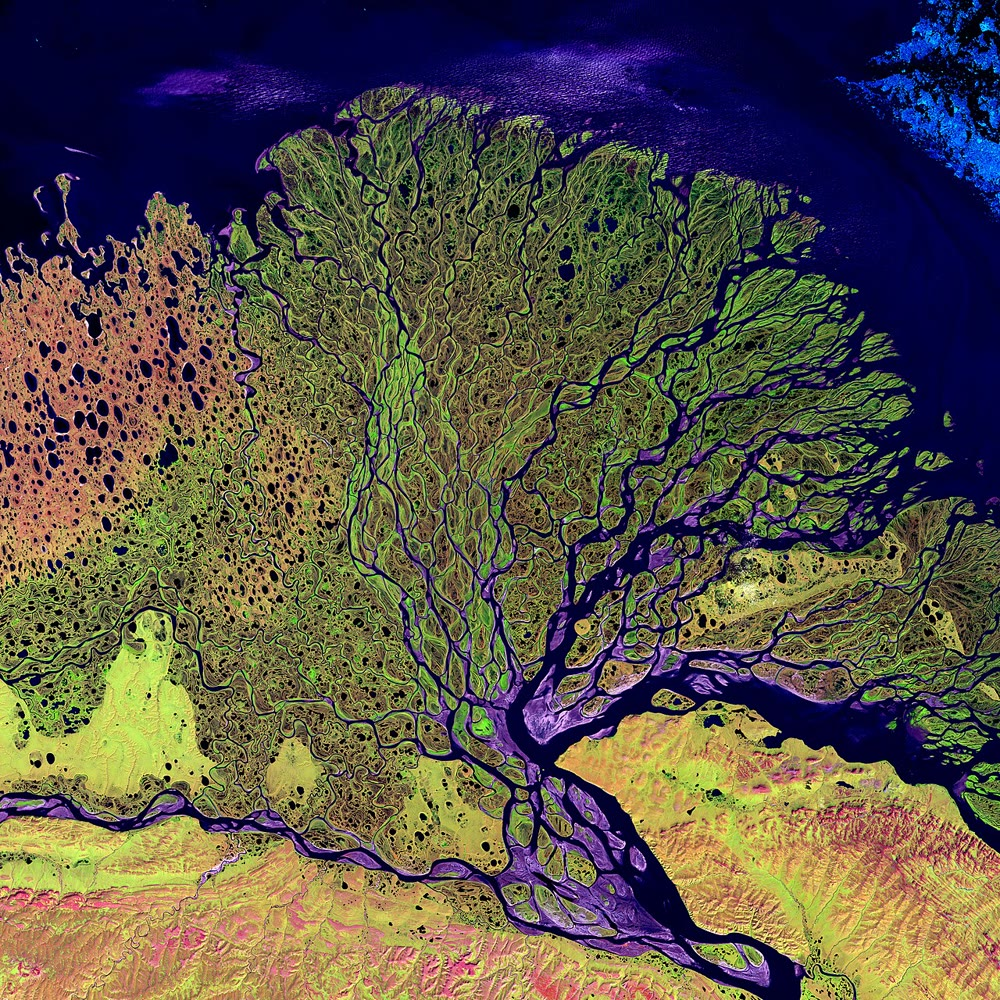
\includegraphics[width=\linewidth]{images/book1/g9-lena-delta.jpg}
\end{minipage}\hfill
\begin{minipage}[c]{0.46\linewidth}\raggedright
{\small The \omterm{def:g5:water-shapes-the-land:delta}{delta} of the \omterm{def:g1:landscapes-around-us:water}{river} Lena, in Siberia, where it meets the Arctic
\omterm{def:g2:water-on-earth:ocean}{Ocean}: a false-colour Landsat image of 27~February 2000, made with
shortwave infrared, infrared and red light. The many channels of the \omterm{def:g1:landscapes-around-us:water}{river}
show in blue. USGS EROS Data Center, via NASA Visible Earth (public domain,
via Wikimedia Commons).}
\end{minipage}
% ledger: commons:lena-landsat
\label{fig:g9:maps-of-the-earth:lena}
\end{omfigure}

\section{Satellite positioning}

A phone or a car can tell where it is to within a few metres, almost
anywhere on the Earth. It does not see the satellites; it listens to them.

\begin{definition}[Satellite positioning]\label{def:g9:maps-of-the-earth:positioning}
\emph{Satellite positioning}\index{satellite positioning} is finding a
position on the Earth from the distances to several satellites whose
positions are known. A receiver computes each distance from the time a
signal from the satellite takes to reach it.
\end{definition}

The American system, GPS, keeps at least 24 working satellites at an
\omterm{def:g4:world-physical-map:altitude}{altitude} of about \qty{20200}{km}. Each circles the Earth twice a day, in
six orbits spread around the planet, so that from almost any point on the
Earth at least four satellites are in view. A signal from \qty{20200}{km}
away, travelling at the speed of light, arrives after $20\,200 \div
300\,000 \approx 0.067$~s: the receiver measures this time and turns it
into a distance.
% ledger: gps:constellation, const:c (travel time computed in figdata/grade-9/trilateration.py)

How do distances give a position? Picture the idea on a flat \omterm{def:g2:drawing-to-map:map}{map}. If the
receiver is \qty{5}{km} from beacon~A, it lies somewhere on a circle of
radius \qty{5}{km} around A. If it is also \qty{10}{km} from B, it lies on
both circles: at one of the two points where they cross. A third distance,
\qty{5}{km} from C, picks the right one. In space, the circles become
spheres, and one more satellite is needed for the same reason.

\begin{omfigure}
\begin{minipage}[c]{0.5\linewidth}\centering
\begin{tikzpicture}
\begin{axis}[x=0.42cm, y=0.42cm, xmin=-1, xmax=13, ymin=-1.5, ymax=13,
  ticks=none, axis line style={black!40}]
  \addplot[omSea!70!black, line width=0.6pt] table {figdata/out/grade-9-trilateration-circles.dat};
  \addplot[only marks, mark=triangle*, mark size=2.6pt, point meta=explicit symbolic, nodes near coords,
    nodes near coords style={font=\footnotesize\bfseries, anchor=south west, inner sep=1pt}]
    table[meta=label] {figdata/out/grade-9-trilateration-beacons.dat};
  % labels first (on a white patch), then the points on top of them
  \addplot[only marks, mark=none, point meta=explicit symbolic, nodes near coords,
    nodes near coords style={font=\footnotesize\bfseries, anchor=north east, xshift=-1pt, yshift=-1pt, inner sep=1pt, fill=white, text=red!75!black}, skip coords between index={1}{2}]
    table[meta=label] {figdata/out/grade-9-trilateration-points.dat};
  \addplot[only marks, mark=none, point meta=explicit symbolic, nodes near coords,
    nodes near coords style={font=\footnotesize, anchor=south west, xshift=1pt, yshift=1pt, inner sep=1pt, fill=white}, skip coords between index={0}{1}]
    table[meta=label] {figdata/out/grade-9-trilateration-points.dat};
  \addplot[only marks, mark=*, mark size=2pt, red!75!black, skip coords between index={1}{2}] table {figdata/out/grade-9-trilateration-points.dat};
  \addplot[only marks, mark=o, mark size=2pt, fill=white, skip coords between index={0}{1}] table {figdata/out/grade-9-trilateration-points.dat};
\end{axis}
\end{tikzpicture}
\end{minipage}\hfill
\begin{minipage}[c]{0.46\linewidth}\raggedright
{\small Positioning on a flat \omterm{def:g2:drawing-to-map:map}{map} (a sketch; grid in kilometres not drawn).
The receiver R is \qty{5}{km} from A, \qty{10}{km} from B and \qty{5}{km}
from C. The circles around A and B cross at R and at a false point F; only
R also lies on the circle around C.}
\end{minipage}
% ledger: (invented region: exercise data, figdata/grade-9/trilateration.py)
\label{fig:g9:maps-of-the-earth:trilateration}
\end{omfigure}

\begin{omfigure}
\begin{minipage}[t]{0.48\linewidth}\centering
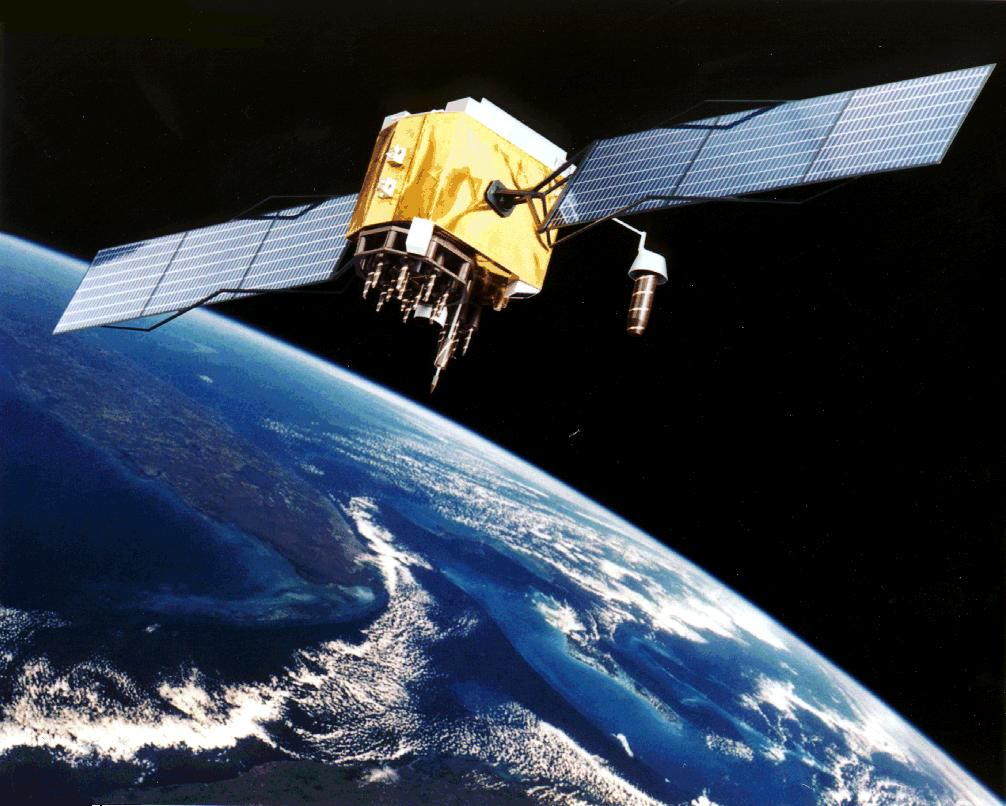
\includegraphics[width=\linewidth]{images/book1/g9-gps-satellite.jpg}

{\small A GPS satellite in orbit, as an artist pictured it. NASA (public
domain, via Wikimedia Commons).}
\end{minipage}\hfill
\begin{minipage}[t]{0.48\linewidth}\centering
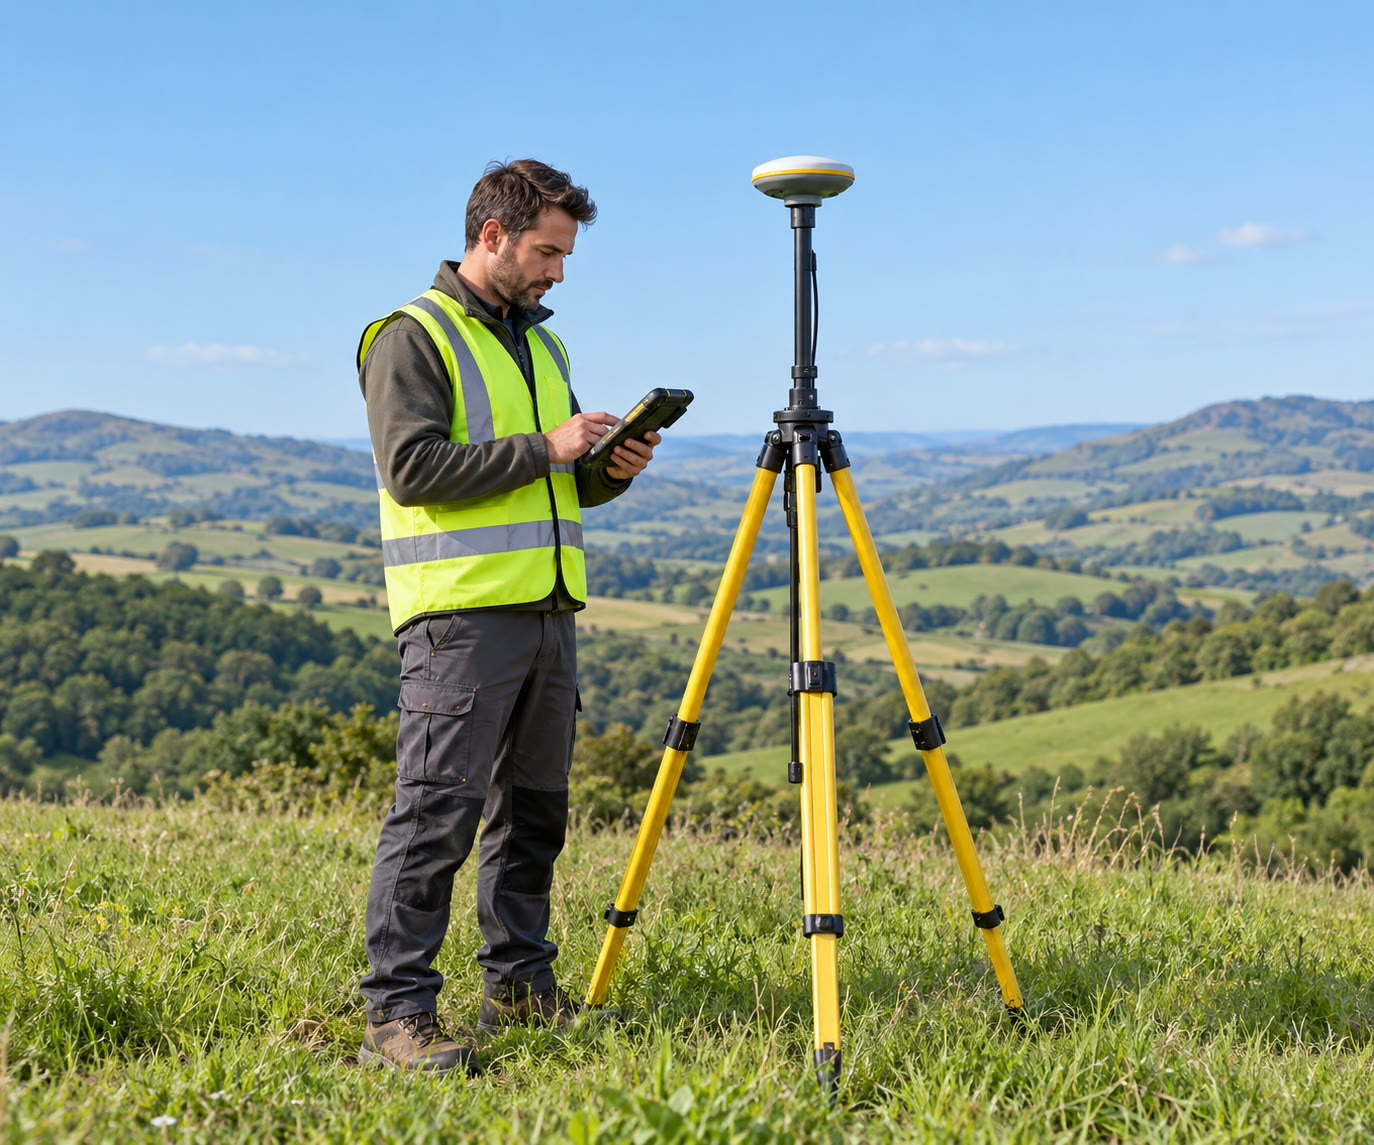
\includegraphics[width=\linewidth]{images/book1/ai/g9-surveyor.jpg}

{\small A surveyor fixes the position of a point with a satellite receiver
on a tripod (an illustration).}
\end{minipage}
% ledger: commons:gps-iif
\label{fig:g9:maps-of-the-earth:gps}
\end{omfigure}

\section{Exercises}

\begin{exercise}[$\star$]\label{exo:g9:maps-of-the-earth:1}
Give the word for each description. (a) A rule that sends each point of
the \omterm{def:g3:continents-and-oceans:globe}{globe} to a point of a flat \omterm{def:g2:drawing-to-map:map}{map}. (b) A line joining points at the same
\omterm{def:g4:world-physical-map:altitude}{altitude}. (c) A ratio such as $1 : 50\,000$. (d) The difference in
\omterm{def:g4:world-physical-map:altitude}{altitude} between two neighbouring \omterm{def:g9:maps-of-the-earth:contour}{contour lines}. (e) Observing the Earth
from a distance, for example from a satellite.
\end{exercise}

\begin{exercise}[$\star$]\label{exo:g9:maps-of-the-earth:2}
Convert each \omterm{def:g2:drawing-to-map:map}{map} distance into a distance on the ground, in metres or
kilometres. (a) \qty{4}{cm} on a $1 : 25\,000$ \omterm{def:g2:drawing-to-map:map}{map}. (b) \qty{3}{cm} on a
$1 : 50\,000$ \omterm{def:g2:drawing-to-map:map}{map}. (c) \qty{2.5}{cm} on a $1 : 1\,000\,000$ \omterm{def:g2:drawing-to-map:map}{map}. (d) On a
$1 : 25\,000$ \omterm{def:g2:drawing-to-map:map}{map}, how many centimetres stand for \qty{1}{km}?
\end{exercise}

\begin{exercise}[$\star$]\label{exo:g9:maps-of-the-earth:3}
True or false? Correct the false sentences. (a) A \omterm{def:g3:continents-and-oceans:world-map}{world map} can show the
whole Earth without distorting anything. (b) On a Mercator \omterm{def:g2:drawing-to-map:map}{map}, Greenland
looks bigger than it is. (c) On an equal-area \omterm{def:g2:drawing-to-map:map}{map}, shapes are kept
everywhere. (d) A \omterm{def:g9:maps-of-the-earth:numerical-scale}{scale bar} stays right when a \omterm{def:g2:drawing-to-map:map}{map} is enlarged on a
copier.
\end{exercise}

\begin{exercise}[$\star$]\label{exo:g9:maps-of-the-earth:4}
On a \omterm{def:g9:maps-of-the-earth:topographic-map}{topographic map}, (a) what does it mean when \omterm{def:g9:maps-of-the-earth:contour}{contour lines} are very
close together? (b) far apart? (c) What do closed \omterm{def:g9:maps-of-the-earth:contour}{contour lines} rising
inwards show? (d) Why can two \omterm{def:g9:maps-of-the-earth:contour}{contour lines} never cross?
\end{exercise}

\begin{exercise}[$\star\star$]\label{exo:g9:maps-of-the-earth:5}
% ledger: data:ne-land (factor 1/cos^2, figdata/grade-9/projections.py)
On a Mercator \omterm{def:g2:drawing-to-map:map}{map}, areas at \omterm{def:g6:latitude-longitude:latitude}{latitude} \ang{60} are enlarged 4 times, and at
\omterm{def:g6:latitude-longitude:latitude}{latitude} \ang{30} about 1.33 times, compared with the \omterm{def:g3:continents-and-oceans:equator}{equator}. (a) A \omterm{def:g1:landscapes-around-us:water}{lake}
of \qty{1000}{km^2} at \ang{60}\,N is drawn on the \omterm{def:g2:drawing-to-map:map}{map}. A \omterm{def:g1:landscapes-around-us:water}{lake} at the
\omterm{def:g3:continents-and-oceans:equator}{equator} drawn with the same size has what true area? (b) Two islands of
the same true area lie at \ang{30} and at \ang{60}. How many times larger
does the second look than the first? (c) Why can the Mercator \omterm{def:g2:drawing-to-map:map}{map} never
show the \omterm{def:g3:continents-and-oceans:poles}{poles}?
\end{exercise}

\begin{exercise}[$\star\star$]\label{exo:g9:maps-of-the-earth:6}
% ledger: (invented region: the Varden Hills map of the chapter)
Use the \omterm{def:g9:maps-of-the-earth:topographic-map}{topographic map} of the Varden Hills in this chapter. (a) What is
the \omterm{def:g9:maps-of-the-earth:contour}{contour interval}? (b) What is the \omterm{def:g4:world-physical-map:altitude}{altitude} of the summit marked by its
spot height, and of the index contour just around it? (c) The \omterm{def:g1:landscapes-around-us:water}{river} flows
east. Is the \omterm{def:g1:landscapes-around-us:landform}{valley} floor higher in the west or in the east of the \omterm{def:g2:drawing-to-map:map}{map}?
(d) Along C--D, north of the \omterm{def:g1:landscapes-around-us:water}{river}, between which \omterm{def:g9:maps-of-the-earth:contour}{contour lines} are the
lines closest together? What does that tell you about the slope there?
\end{exercise}

\begin{exercise}[$\star\star$]\label{exo:g9:maps-of-the-earth:7}
% ledger: (invented region: profile C--D, figdata/grade-9/varden_topo.py)
Use the profile C--D in this chapter. (a) At about what \omterm{def:g4:world-physical-map:altitude}{altitude} are C
and D? (b) What is the lowest \omterm{def:g4:world-physical-map:altitude}{altitude} along the profile, and how far from
C is it? (c) How long is the flat \omterm{def:g1:landscapes-around-us:landform}{valley} floor along C--D? (d) The profile
is drawn with its vertical scale stretched three times. Why do mapmakers
often do this?
\end{exercise}

\begin{exercise}[$\star\star$]\label{exo:g9:maps-of-the-earth:8}
On a $1 : 25\,000$ \omterm{def:g2:drawing-to-map:map}{map}, a path crosses the \qty{200}{m} contour and then
the \qty{300}{m} contour, \qty{2}{cm} further on. (a) What is the
horizontal distance between the two points on the ground? (b) How much
does the path climb? (c) What is the slope, as a percentage? (d) Further
on, two contours \qty{100}{m} apart in \omterm{def:g4:world-physical-map:altitude}{altitude} are \qty{4}{cm} apart on the
\omterm{def:g2:drawing-to-map:map}{map}. Is the path steeper or gentler there? By how much?
\end{exercise}

\begin{exercise}[$\star\star$]\label{exo:g9:maps-of-the-earth:9}
% ledger: usgs:landsat1
Landsat~1 circled the Earth 14 times a day and passed over the same place
every 18 days. (a) How many orbits did it make between two passes over the
same place? (b) Each orbit took 103 minutes. How long, in hours, are 14
orbits? (c) Built to work one year, it was switched off on 6~January 1978,
five and a half years after its launch. How many times its planned life did
it work? (d) Give one change on the Earth's surface that images of the same
place taken years apart can show.
\end{exercise}

\begin{exercise}[$\star\star$]\label{exo:g9:maps-of-the-earth:10}
% ledger: gps:constellation, const:c
A GPS satellite is about \qty{20200}{km} away; its signal travels at
about \qty{300000}{km} per second. (a) How long does the signal take to
arrive? Write the answer in scientific notation. (b) If a receiver's
clock were wrong by $1 \times 10^{-3}$~s, what error in the distance would
that make? (c) What does this tell you about the clocks used in \omterm{def:g9:maps-of-the-earth:positioning}{satellite
positioning}?
\end{exercise}

\begin{exercise}[$\star\star\star$]\label{exo:g9:maps-of-the-earth:11}
On a flat \omterm{def:g2:drawing-to-map:map}{map} with a grid in kilometres, beacon A is at $(0, 0)$ and
beacon B at $(10, 0)$. A receiver is \qty{6}{km} from A and \qty{8}{km}
from B. (a) Show that the point $(3.6, 4.8)$ is \qty{6}{km} from A and
\qty{8}{km} from B. (b) Give another point at the same distances from A
and B. (c) A third beacon C is at $(0, 10)$, and the receiver is about
\qty{6.3}{km} from it. Which of the two points is the receiver? (d) Why
does \omterm{def:g9:maps-of-the-earth:positioning}{satellite positioning} need several satellites?
\end{exercise}

\begin{exercise}[$\star\star\star$]\label{exo:g9:maps-of-the-earth:12}
% ledger: data:ne-land (areas, figdata/grade-9/projections.py)
Africa's mainland covers about 29~million~\unit{km^2} and Greenland about
2.1~million~\unit{km^2}. (a) How many times larger is Africa? (b) On a
Mercator \omterm{def:g2:drawing-to-map:map}{map}, areas near the middle of Greenland, at about \ang{72}\,N,
are enlarged about 10.5 times. Estimate the area Greenland seems to have.
(c) Africa lies across the \omterm{def:g3:continents-and-oceans:equator}{equator}, where areas are enlarged little.
Compare your answer to (b) with Africa's area, and explain the wall \omterm{def:g2:drawing-to-map:map}{map} of
the start of the chapter. (d) Which projection would you choose to show
the sizes of the \omterm{def:g3:continents-and-oceans:continent}{continents} fairly?
\end{exercise}

\section{Problem: A footpath across the Varden Hills}

\begin{problem}[{Weekend problem --- planners have drawn a footpath across
the Varden Hills on the topographic map; the final answer is the length of
the footpath in kilometres and its total climb in metres}]
\label{pb:g9:maps-of-the-earth:1}
% ledger: (invented region: the Varden Hills, figdata/grade-9/varden_topo.py, part problem: leg lengths 3.6 / 2.5 / 2.35 cm, spot heights 296 / 143 / 335 / 544 m, 4.2 km, 401 m)
The footpath starts at a farm S, goes down to a bridge B over the \omterm{def:g1:landscapes-around-us:water}{river},
then climbs to a shelter W and on to the summit T. Each leg is straight and
only goes down or only goes up. The \omterm{def:g2:drawing-to-map:map}{map} is at $1 : 50\,000$; the \omterm{def:g4:world-physical-map:altitude}{altitudes}
of S, B, W and T are written beside them.

\begin{omfigure}
\begin{tikzpicture}
\begin{axis}[x=1.6cm, y=1.6cm, xmin=2, xmax=8, ymin=1.8, ymax=6.2, ticks=none,
  axis line style={black!60}, clip mode=individual]
  \addplot[contour] table {figdata/out/shared-region-contours.dat};
  \addplot[index contour] table {figdata/out/shared-region-index-contours.dat};
  \addplot[river] table {figdata/out/shared-region-river.dat};
  \addplot[only marks, mark=none, point meta=explicit symbolic, nodes near coords,
    nodes near coords align={center}, nodes near coords style={font=\tiny, fill=white, inner sep=0.6pt, text=omContour}]
    table[meta=label] {figdata/out/grade-9-varden_topo-labels.dat};
  \addplot[red!75!black, line width=1pt, dashed] table[x=x_km, y=y_km] {figdata/out/grade-9-varden_topo-path.dat};
  \addplot[only marks, mark=*, mark size=1.6pt, red!75!black, point meta=explicit symbolic, nodes near coords,
    nodes near coords align={right}, nodes near coords style={font=\scriptsize\bfseries, text=black, fill=white, fill opacity=0.8, text opacity=1, inner sep=1pt}]
    table[meta=label] {figdata/out/grade-9-varden_topo-points.dat};
  \coordinate (na) at (axis cs:8.35,5.4);
\end{axis}
\pic at (na) {northarrow};
\end{tikzpicture}

{\small The footpath S--B--W--T on the \omterm{def:g9:maps-of-the-earth:topographic-map}{topographic map} of the Varden Hills
(shown here reduced; on the original \omterm{def:g2:drawing-to-map:map}{map} at $1 : 50\,000$ the legs measure
3.6, 2.5 and \qty{2.35}{cm}).}
\label{fig:g9:maps-of-the-earth:path}
\end{omfigure}

\noindent\textbf{Part I --- The route on the map.}\par\nopagebreak
\begin{enumerate}[beginpenalty=10000]
  \item At $1 : 50\,000$, how many metres on the ground does \qty{1}{cm}
        of the \omterm{def:g2:drawing-to-map:map}{map} stand for?
  \item On the original \omterm{def:g2:drawing-to-map:map}{map}, the leg S--B measures \qty{3.6}{cm}. How
        long is it on the ground, in kilometres?
  \item The legs B--W and W--T measure \qty{2.5}{cm} and \qty{2.35}{cm}.
        How long are they on the ground?
  \item In which general direction does the path run from B to T?
\end{enumerate}

\noindent\textbf{Part II --- The climb.}\par\nopagebreak
\begin{enumerate}[resume, beginpenalty=10000]
  \item What is the \omterm{def:g9:maps-of-the-earth:contour}{contour interval} of the \omterm{def:g2:drawing-to-map:map}{map}?
  \item Which leg goes down? By how many metres?
  \item By how many metres does the path climb on B--W, and on W--T?
  \item What is the average slope of the leg W--T, as a percentage?
  \item Why did the planners not draw the path in a straight line from S
        to T?
\end{enumerate}

\noindent\textbf{Part III --- The walk.}\par\nopagebreak
\begin{enumerate}[resume, beginpenalty=10000]
  \item Suppose a walker covers \qty{4}{km} an hour on the flat and needs
        one more minute for every \qty{10}{m} of climb. How long does the
        whole walk take?
  \item Another walker follows the footpath the other way, from T to S.
        How many metres does she climb?
  \item What is the total length of the footpath, in kilometres, and its
        total climb, in metres?
\end{enumerate}
\end{problem}
